\documentclass[]{beamer}

\usepackage{fontspec} 
% \usepackage{lsp-makros}
\useoutertheme{lsp}

\usepackage{lsptitle}

\def\two@digits#1{\ifnum#1<10 0\fi\number#1}
\def\mytoday{\two@digits{\number\day}.\two@digits{\number\month}.\number\year}


\usepackage{xspace,multicol}
\newcommand{\latex}{\LaTeX\xspace}
\usepackage{tikz}


\newcounter{lastpagemainpart}
\footnotesep0pt
\renewcommand{\footnoterule}{}
\usefootnotetemplate{
  \noindent
  \insertfootnotemark\insertfootnotetext}

\let\beamerfn=\footnote
\renewcommand{\footnote}[1]{%
\let\oldfnsize=\footnotesize%
\let\footnotesize=\tiny%
\beamerfn<\thebeamerpauses->{#1}%
\let\footnotesize=\oldfnsize}


\date{\today}

\usepackage{eurosym}  
 
\renewcommand{\centerline}[1]{\hfill#1\hfill\hfill\mbox{}}
\newcommand{\highlight}{\mdseries\color{red!80!black}}

\title{How to turn your thesis into an accessible book}
% \institute{FU Berlin}
\author[Nordhoff]{Sebastian Nordhoff}
\date{STaPs 17, 2021-04-21}


\begin{document}
\lspbeamertitle

\section{Introduction}

% \frame{
% \frametitle{Outline}
% \tableofcontents
% }

\frame{
\frametitle{Sebastian Nordhoff}
%   \includegraphics[height=.2\textheight]{./path/to/graphicsfile}
  \begin{itemize}
    \item PhD 2009 \textit{A grammar of Upcountry Sri Lanka Malay}
    \item 3 edited volumes, about 30 research articles
    \item 2009-2012 Glottolog.org at the Max Planck Institute for Evolutionary Anthropology
    \item advocate for Open Source, Open Access, Open Data, Open Everything 
    \item since 2014 coordinator for Language Science Press
    \item involved in the publication of 150+ books since 2014
    \begin{itemize}
      \item maybe 30 of them based on theses
    \end{itemize}

  \end{itemize}
}

\frame{
\frametitle{Language Science Press}
%   \includegraphics[height=.2\textheight]{./path/to/graphicsfile}
  \begin{itemize}
    \item  scholar-owned, community-based publisher 
    \item Open Access
    \item free to read 
    \item free to publish 
    \item 29 series
    \item 30 books a year (monographs and edited volumes)
    \item Open-Access-Preis of the Deutsche Gesellschaft für Sprachwissenschaft 2018
  \end{itemize}
}

\frame{
\frametitle{Language Science Press}
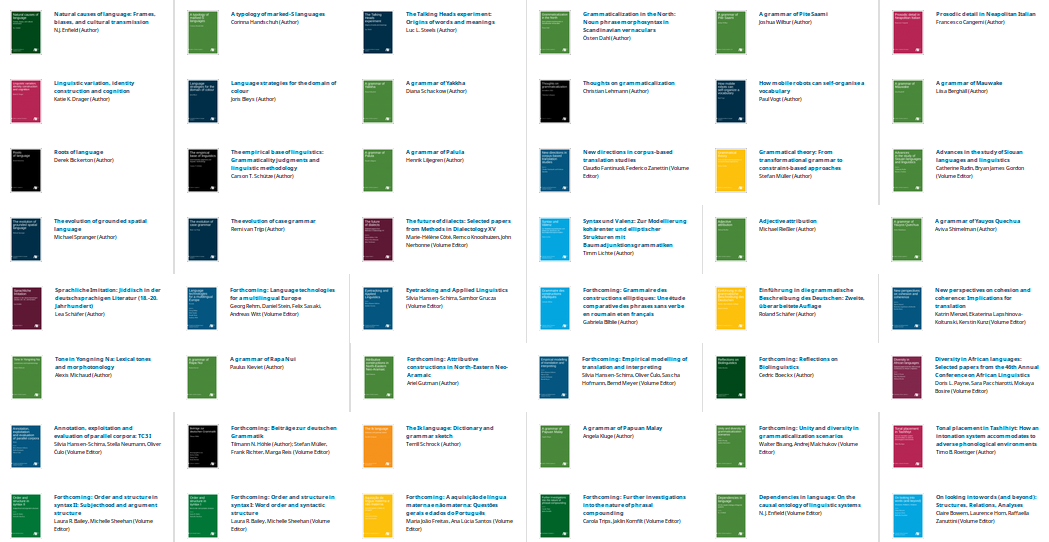
\includegraphics[height=\textheight]{catalog.png}
}
% 
% \frame{
% \frametitle{Production of a book:\\ traditional model}
% %   \includegraphics[height=.2\textheight]{./path/to/graphicsfile}
%   \begin{enumerate}
%     \item inquiry
% 	\item book proposal
% 	\item proposal approval
% 	\item contract
% 	\item first submission
% 	\item review
% 	\item first decision
% 	\item revision
% 	\item final decision
% 	\item copyediting
% 	\item first proofs
% 	\item typesetting
% 	\item final proofs
%   \end{enumerate}
% }


\section{Thesis $\to$ book}
\frame{
\frametitle{Thesis $\to$ book}
%   \includegraphics[height=.2\textheight]{./path/to/graphicsfile}
  \begin{itemize}
    \item  Select series
    \item Contact series editors
    \item Discuss how the book would fit into the series
    \item De-dissertationize
    \begin{itemize}
      \item shorten ``history of research''.
      \item footnotes are not a sign of erudition. Drop/shorten as much as you can.
    \end{itemize}
    \item wait for reviews
    \item revision, copyediting, typesetting.
  \end{itemize}
}



            
\section{Legal aspects}

\frame{
\frametitle{Access and copyright}
%   \includegraphics[height=.2\textheight]{./path/to/graphicsfile}
  \begin{itemize}
    \item  ``Copyright'' in the Anglo-Saxon countries
    \item  ``Urheberrecht'' in continental Europe 
    \item These are different!
    \item Once you create something, you can decide who can use it and how
    \item Choose wisely and be explicit!
  \end{itemize}
}

\frame{
\frametitle{License}
%   \includegraphics[height=.2\textheight]{./path/to/graphicsfile}
  \begin{itemize}
    \item  Usage rights can be differentiated as follows
    \begin{itemize}
      \item geographical restriction (e.g. \textit{only for Germany})
      \item type restrictions (e.g. \textit{only for print}) 
      \item exclusive (no-one else has the right) vs. non-exclusive (other people may also get the rights)
      \item copyright transfer agreement (Anglo-Saxon culture)
      \item total buy-out
    \end{itemize}
  \end{itemize}
}

\frame{
\frametitle{Copyright transfer agreement}
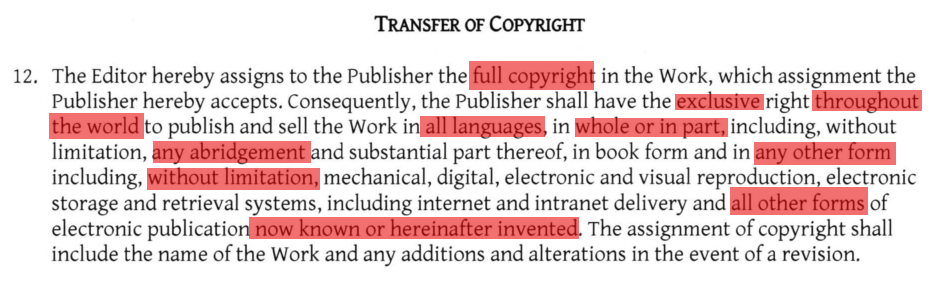
\includegraphics[width=\textwidth]{copyrighttransfer.pdf}
}

\frame{
\frametitle{Contracts}
%   \includegraphics[height=.2\textheight]{./path/to/graphicsfile}
  \begin{itemize}
    \item  Publisher contracts restrict everybody, including yourself 
    \item once you sign away your copyright, you have \textbf{no longer the right to use your own material}
    \begin{itemize}
      \item it is possible to keep your copyright, depending on the publisher. Language Science Press requires a non-exclusive license only, no copyright transfer
    \end{itemize}
    \item to reuse  graphics in subsequent works of yours, you must first ask the new rights holder for permission
    \item chasing rights is incredibly annoying
    \item publishers will put your content behind a \textbf{paywall}, meaning that it can actually be more difficult to access once it is officially published than before
    \item publishers vary as to whether and when they allow books to be hosted in repositories
    \item check \textbf{Sherpa-Romeo} \url{https://v2.sherpa.ac.uk/romeo/}, which lists the publishers' policies
  \end{itemize}
    }

\frame{
\frametitle{Availability of Nordhoff (ed.) (2012)}
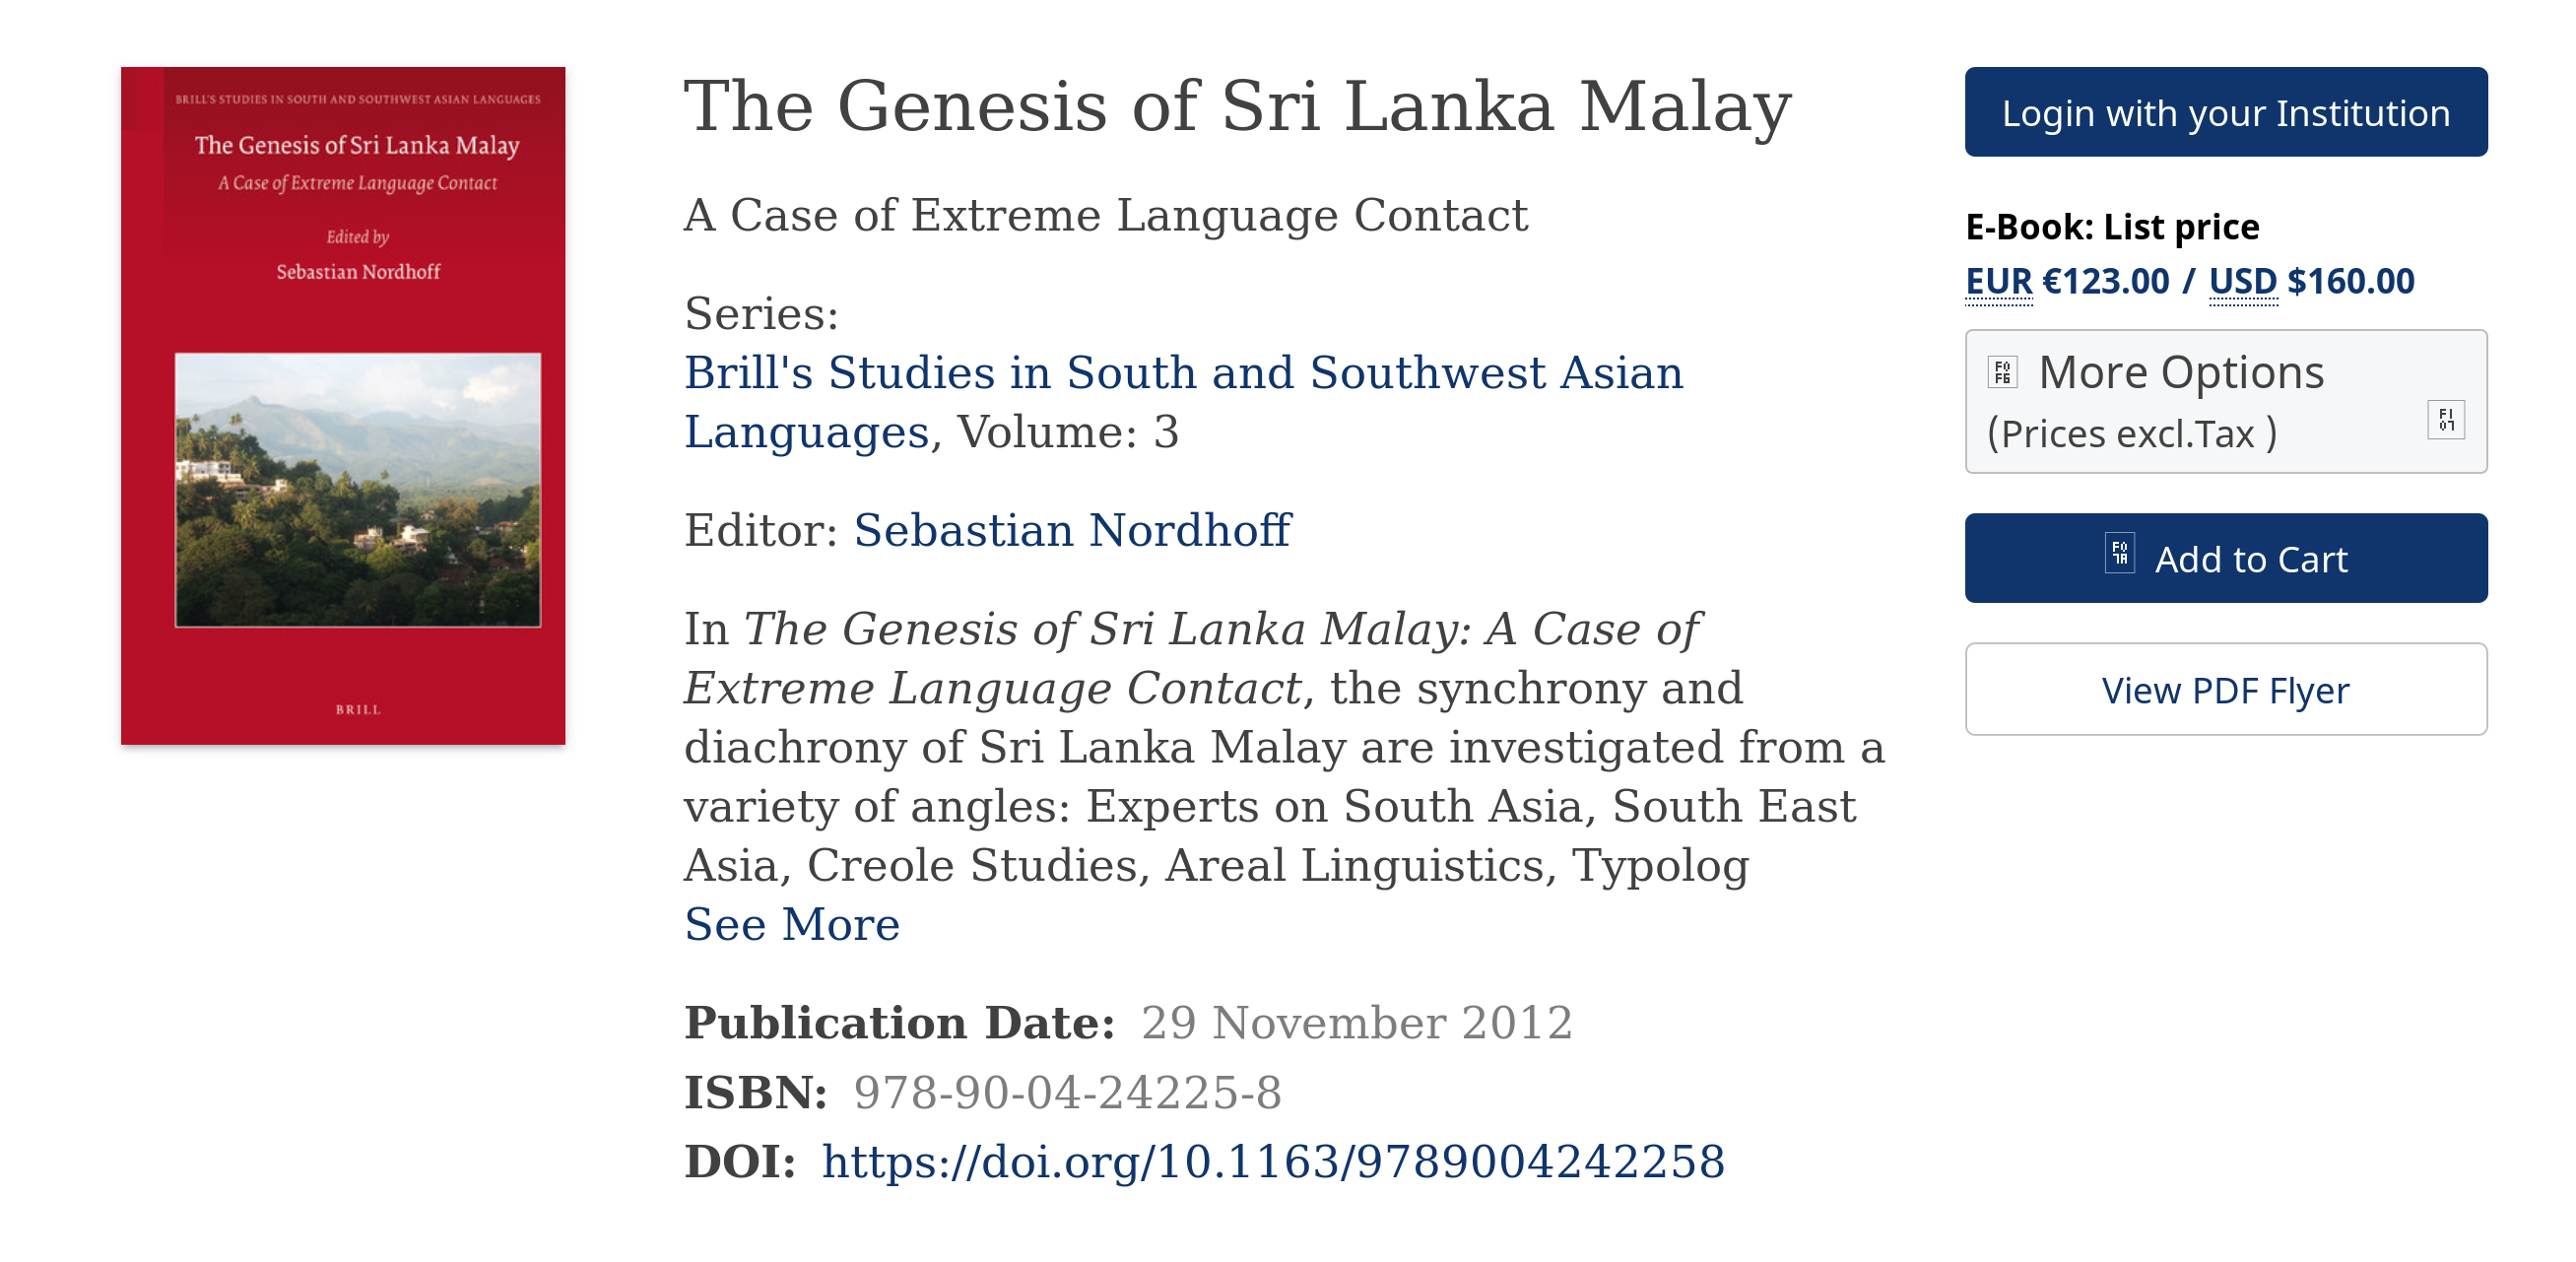
\includegraphics[width=\textwidth]{brillnordhoff.png}
 }

\frame{ 
\frametitle{Licensing recommendations}
  \begin{itemize}
    \item Publish your works under a Creative Commons license, \textbf{preferably CC-BY}
    \item This license clearly states who the copyright holder is and how the content can be reused (typically requiring only the attribution of the original author)
    \item see Fair Open Access principles on \url{https://www.lingoa.eu/about/mission}
    \item do not sign away your copyright
    \begin{itemize}
      \item You can also ``prepublish'' ``your'' version under CC-BY in an archive before signing the author contract with a publisher
      \item This is called the \textbf{Rights Retention Strategy}
      \item {\scriptsize \url{https://www.coalition-s.org/the-RRS-and-publisher-equivocation-an-open-letter-to-researchers}}
    \end{itemize}
  \end{itemize}
}
                
%                 The editor hereby assigns to the Publisher the full copyright in the Work [...]. Consequently, the Publisher shall have the exclusive right \textbf{throughout the world} to publish and sell th Work in \textbf{all languages}, in whole or in part, including, \textbf{without limitation}, \textbf{any} abridgement and substantial part thereof, in book form and in \textbf{any other form} including, without limitation, mechanical, digital electronic, and visual reproduction, electronic storage and retrieval systems, including internet and intranet delivery and \textbf{all other forms of electronic publication now known or hereinafter invented}. 

       
\frame{
\frametitle{Wrap-up: recommendations\\ \mbox{for sustainable book publications}}
%   \includegraphics[height=.2\textheight]{./path/to/graphicsfile}
  \begin{itemize}
    \item separate data, code, and text 
    \item use a versioning system
    \item backup\\~
    \item publish all your data in appropriate repositories
    \item use preprint servers\\~
    \item use the CC-0 license for data and the CC-BY license for text
    \item do not sign away your copyright\\~
    \item care for your discipline, go for scholar-led community-owned publishers
  \end{itemize}
}
    
\section{Thank you}
\frame{
\frametitle{Thank you}
  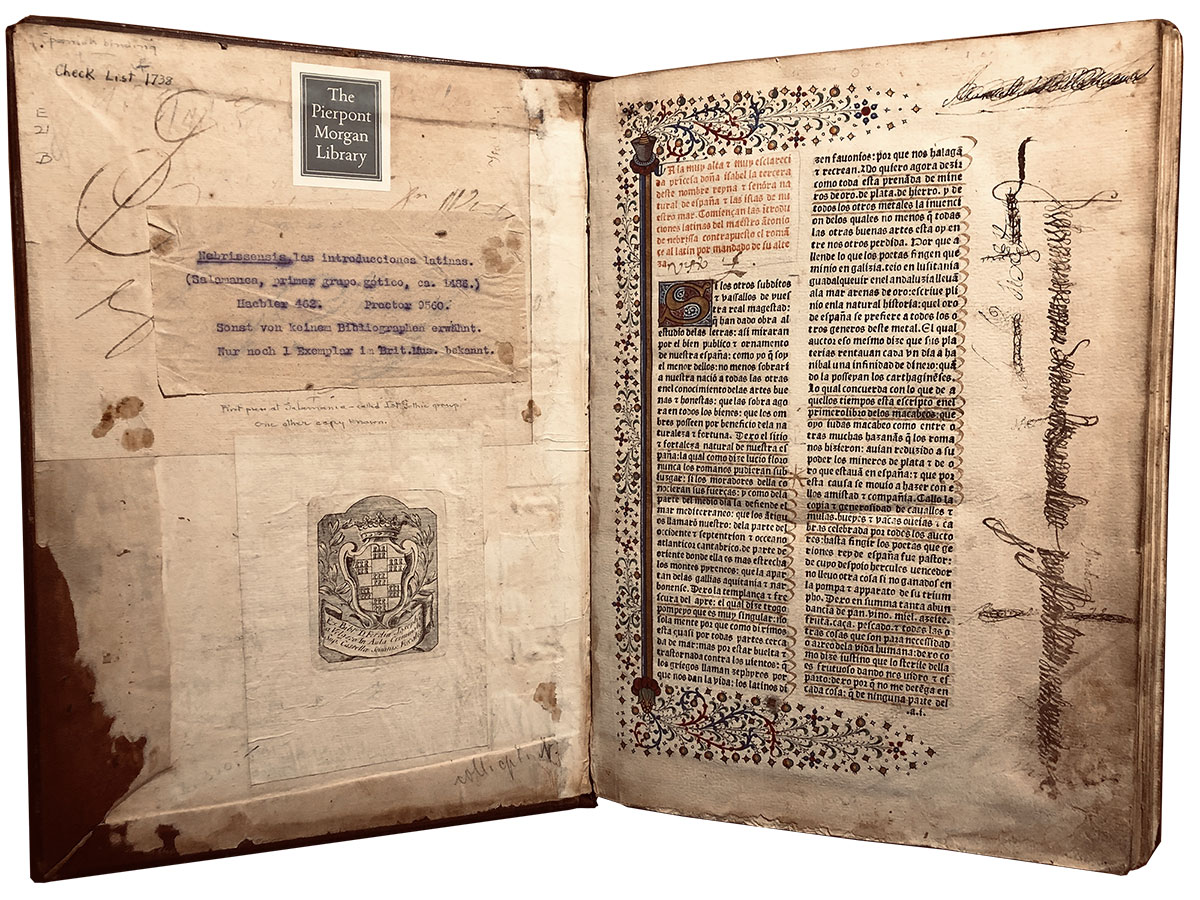
\includegraphics[width=\textwidth]{nebrija.jpg}
}    

\end{document}
